% Chapter 1

\chapter{Introduction} % Main chapter title
\thispagestyle{nohead}
\label{Intro} % For referencing the chapter elsewhere, use \ref{Intro} 

%----------------------------------------------------------------------------------------

% Define some commands to keep the formatting separated from the content 
\newcommand{\keyword}[1]{\textbf{#1}}
\newcommand{\tabhead}[1]{\textbf{#1}}
\newcommand{\code}[1]{\texttt{#1}}
\newcommand{\file}[1]{\texttt{\bfseries#1}}
\newcommand{\option}[1]{\texttt{\itshape#1}}
%----------------------------------------------------------------------------------------

\section{Software Verification Background}
\subsection{Software Verification Systems as Composed of Modular Components}
\subsection{The \why system}
\subsubsection{Front End: \why as an intermediary language}
\subsubsection{Back End: Driver-based interface to \textsc{APT}, \textsc{ITP} and \textsc{SMT} tools}
\section{An overview of various \textsc{SMT} solvers and their capabilities}
\section{The problem we want to solve: the efficient allocation of \textsc{SMT}-solving resources for software verification tasks}
%\section{The benefits of a portfolio-based approach to software verification}
\begin{figure}
\centering
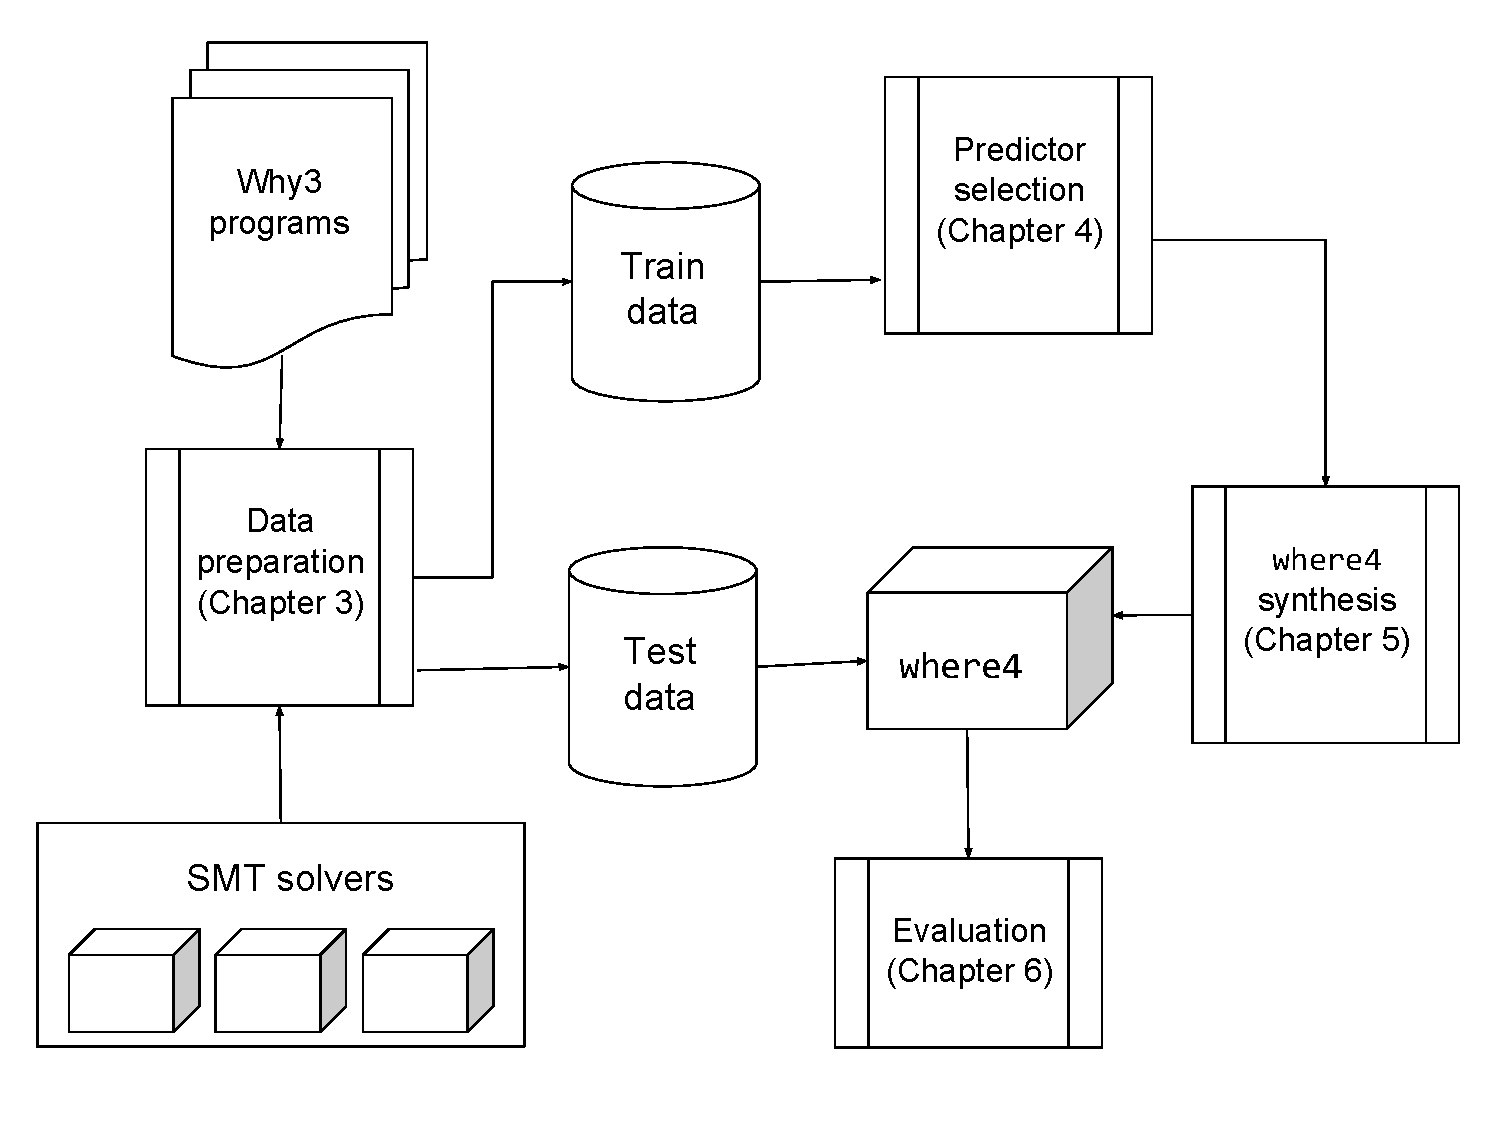
\includegraphics[width=0.9\linewidth]{Figures/intoduction}
\caption{Overview of the \where project and this thesis's structure}
\label{fig:introduction}
\end{figure}

